%& /Users/ziky/.cache/org-persist/a7/872cc4-17cf-49e1-a57c-23fd34f65ebe-28e36686f61ea28d6225596396aff65e
% Created 2025-11-12 Wed 18:58
% Intended LaTeX compiler: pdflatex
\documentclass[11pt]{article}
\usepackage[utf8]{inputenc}
\usepackage[T1]{fontenc}
\usepackage{amsmath}
\usepackage{amssymb}
\usepackage{capt-of}
\usepackage{hyperref}
\setlength{\abovedisplayskip}{0pt}
\setlength{\belowdisplayskip}{0pt}
\usepackage[a4paper, margin=1in]{geometry}
\usepackage{multicol}
\setlength{\columnsep}{1cm}

%% ox-latex features:
%   !announce-start, !guess-pollyglossia, !guess-babel, !guess-inputenc,
%   caption, maths, image, !announce-end.

\usepackage{capt-of}

\usepackage{amsmath}
\usepackage{amssymb}

\usepackage{graphicx}

%% end ox-latex features


% end precompiled preamble
\ifcsname endofdump\endcsname\endofdump\fi

\author{Ziky Zhang}
\date{\today}
\title{Electromagnetism Notes}
\hypersetup{
 pdfauthor={Ziky Zhang},
 pdftitle={Electromagnetism Notes},
 pdfkeywords={},
 pdfsubject={},
 pdfcreator={},
 pdflang={English}}
\begin{document}

\maketitle
\tableofcontents

\newpage
\section{Coulomb's Law}
\label{sec:org683a59a}

\begin{multicols}{2}

\textbf{Charge}, often denoted as $q$. There are two types of charges: positive ($+$) and negative ($-$). \\
Charges of the \underline{same sign repel}, while \underline{opposite signs attract}. \\ \\
Everyday object normally stays neutrually charged, which means that the positively charged particles and negatively charged particles balance out. When this balance breaks, the obkect becomes either positively charged or negatively charged.

\columnbreak

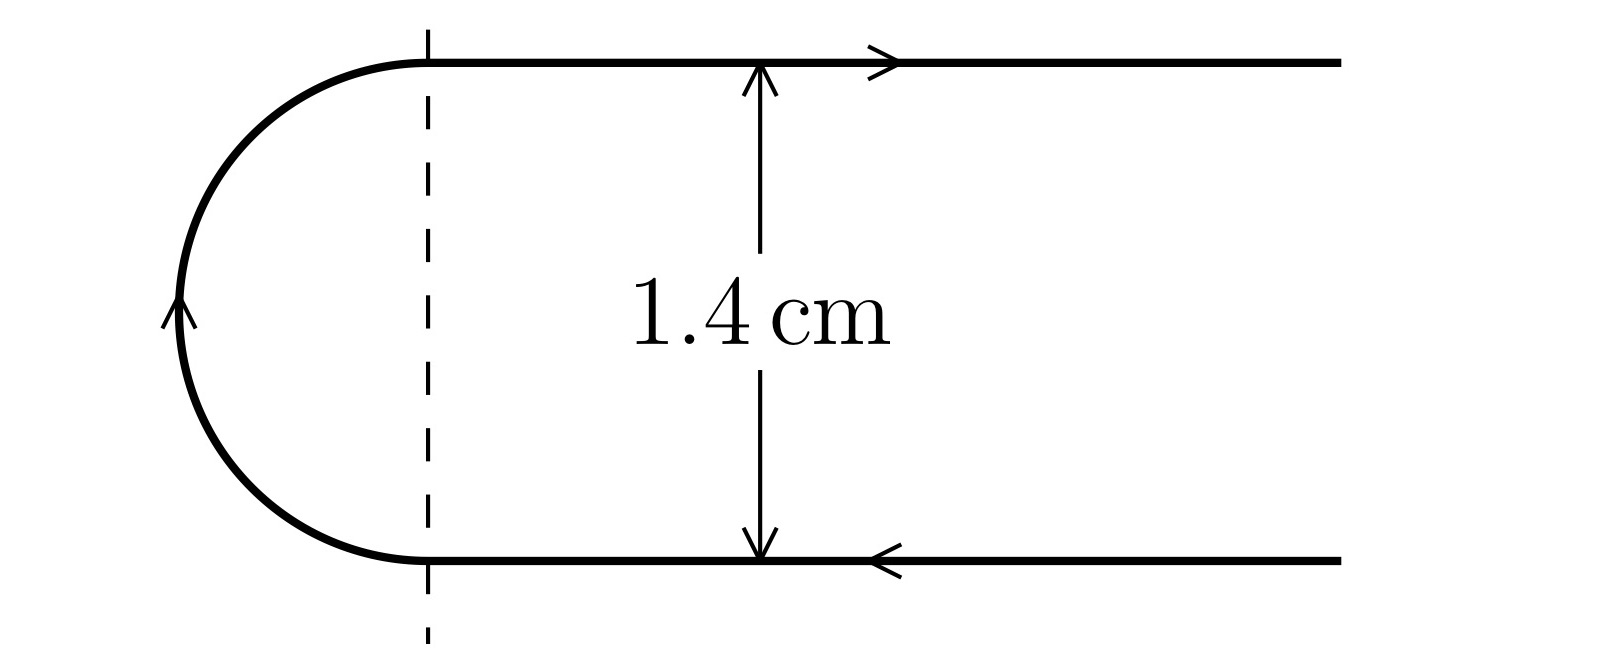
\includegraphics[width=0.9\columnwidth]{./img/10.1.jpg}
\captionof{figure}{Two point charges illustrating attraction and repulsion}

\end{multicols}
\section{}
\label{sec:org010eb3b}

\begin{multicol}2


these are all garbage

\begin{figure}[htbp]
\centering
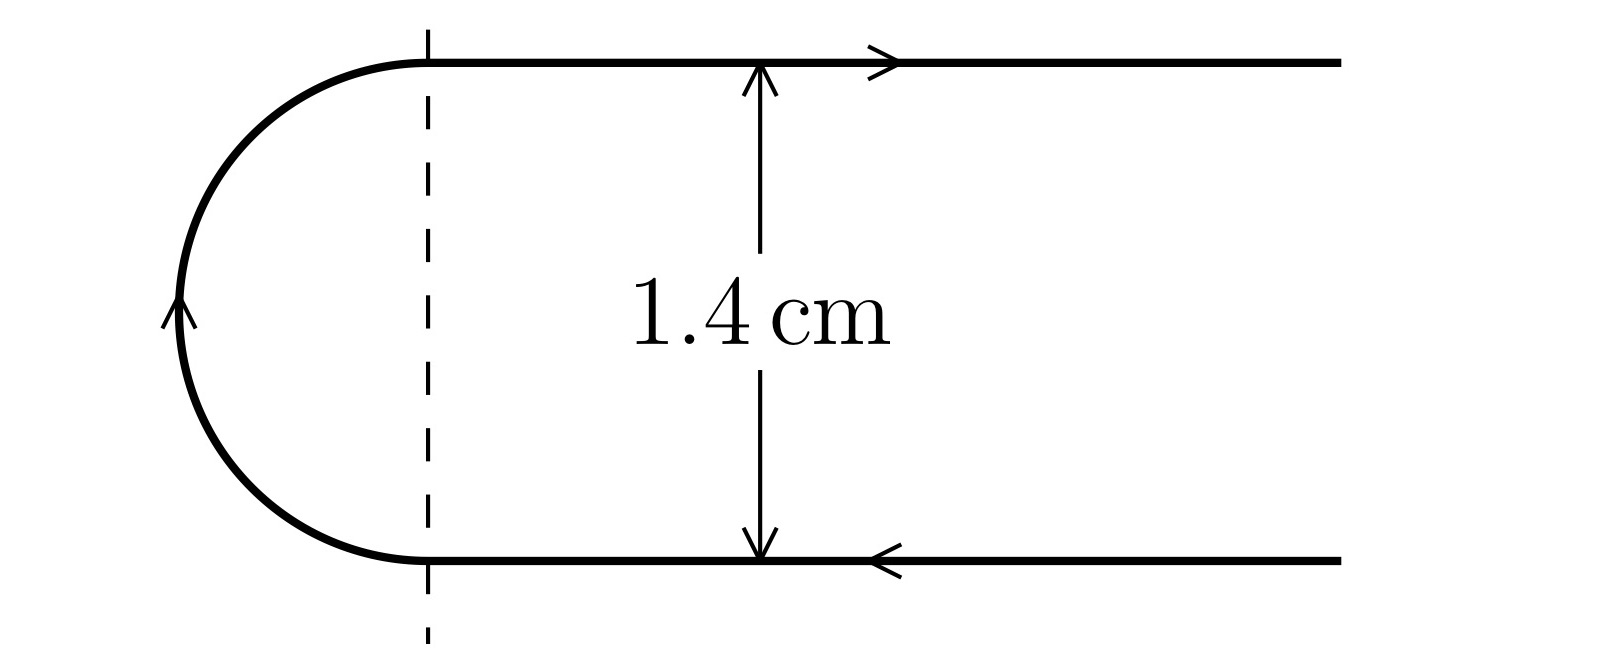
\includegraphics[width=0.9\columnwidth]{./img/10.1.jpg}
\caption{Two point charges hi illustrating attraction and repulsion}
\end{figure}
\end{multicol}
\end{document}
